\documentclass[border=1pt]{standalone}
\usepackage{tikz}
\usepackage{luatexja}

\begin{document}
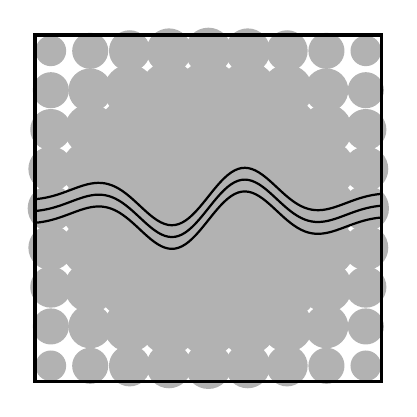
\begin{tikzpicture}
    % 菱形格子のベース
    \foreach \x in {-2,-1.5,...,2} {
        \foreach \y in {-2,-1.5,...,2} {
            % 座標中心からの距離に応じてドットの大きさを変える
            \pgfmathsetmacro{\dotdist}{sqrt(\x*\x + \y*\y)}
            \pgfmathsetmacro{\dotsize}{0.8pt * exp(-0.5*\dotdist)}
            \fill[black!30] (\x, \y) circle (\dotsize);
        }
    }
    % 場の干渉波（中央を貫く力強い線）
    \foreach \h in {-0.15, 0, 0.15} {
        \draw[black, thick, yshift=\h cm] 
            plot[domain=-2.2:2.2, samples=100] (\x, {0.4*sin(deg(pi*\x)) * exp(-0.4*\x*\x)});
    }
    % 幾何学的な枠組み
    \draw[black, very thick] (-2.2, -2.2) rectangle (2.2, 2.2);

\end{tikzpicture}
\end{document}
